\documentclass[11pt,oneside]{article}

% ============================================================
% PACKAGES
% ============================================================
\usepackage[a4paper,margin=1in]{geometry}
\usepackage{amsmath, amssymb, amsthm, mathtools}
\usepackage{microtype}
\usepackage{graphicx}
\usepackage{hyperref}
\usepackage{booktabs}
\usepackage{enumitem}
\usepackage{tikz}
\usetikzlibrary{arrows.meta, positioning, decorations.pathmorphing}
\usepackage[numbers,sort&compress]{natbib}
\usepackage{titlesec}
\usepackage{setspace}

\setstretch{1.16}
\titleformat{\section}{\large\bfseries}{\thesection}{1em}{}
\titleformat{\subsection}{\normalsize\bfseries}{\thesubsection}{1em}{}

% ============================================================
% THEOREM ENVIRONMENTS
% ============================================================
\newtheorem{axiom}{Axiom}
\newtheorem{definition}{Definition}
\newtheorem{theorem}{Theorem}
\newtheorem{lemma}{Lemma}
\newtheorem{proposition}{Proposition}
\newtheorem{corollary}{Corollary}

% ============================================================
% TITLE
% ============================================================
\title{\textbf{Ground Theory:\\
A Complexity--Topological Framework for Quantum, Classical,\\
and Emergent Physics}}

\author{Matthew Scherf}
\date{2025}

\begin{document}
\maketitle
\thispagestyle{empty}

% ============================================================
% ABSTRACT
% ============================================================
\begin{abstract}
\noindent
This monograph develops \emph{Ground Theory}, a unified axiomatic framework
in which quantum, classical, and emergent physical behaviour arise
from a single underlying principle: the algorithmic complexity of states
relative to a minimal six-dimensional Calabi--Yau substrate.
The theory integrates ideal Kolmogorov complexity, operational
Lempel--Ziv approximations, topological invariants, and a grounding relation
that connects measurement, decoherence, and emergence.

A central result is the derivation of the quantum--classical boundary:
the complexity threshold separating coherent (quantum) states from
decoherent (classical) ones equals the topological complexity of the
unique substrate manifold, computed as
\[
c_{\rm grounding} = K_{\rm topo}(M_{\rm substrate}) = 57~\text{bits}.
\]
This boundary is not an empirical fit but a topological necessity.
Additional derived predictions include inseparability constraints,
a complexity-theoretic account of time symmetry breaking,
and---via the Atiyah--Singer index theorem---the existence of exactly
three fermion generations.

The monograph is written for physicists and mathematicians alike:
formally rigorous yet conceptually accessible.
\end{abstract}

\newpage

% ============================================================
% PREFACE
% ============================================================
\section*{Preface}
\addcontentsline{toc}{section}{Preface}

These notes present the 2025 canonical formulation of Ground Theory.
The work is motivated by a simple question: \emph{if reality is made of
information, what determines the boundary between quantum behaviour, classical
behaviour, and emergent structure?}

Rather than treating this boundary as contingent on environment size,
temperature, or arbitrary coarse-graining, the theory isolates a single
mathematically derived threshold---the algorithmic complexity of a uniquely
selected Calabi--Yau substrate manifold.
The resulting framework is minimal, falsifiable, and surprisingly predictive.

The exposition begins with foundational ontology and complexity theory,
then develops the axiomatic structure, the topological foundations,
and the derived predictions.

\newpage

% ============================================================
% TABLE OF CONTENTS
% ============================================================
\tableofcontents
\newpage

%%%%%%%%%%%%%%%%%%%%%%%%%%%%%%%%%%%%%%%%%%%%%%%%%%%%%%%%%%%%%%
% PART I — FOUNDATIONS OF THE FRAMEWORK
%%%%%%%%%%%%%%%%%%%%%%%%%%%%%%%%%%%%%%%%%%%%%%%%%%%%%%%%%%%%%%
\section*{Part I: Foundations of the Framework}
\addcontentsline{toc}{section}{Part I: Foundations of the Framework}

% ============================================================
% CHAPTER 1
% ============================================================
\section{Introduction and Motivation}

The quantum--classical transition remains one of the deepest open problems
in physics.
Decoherence theory, many-worlds interpretations, collapse models,
and gravitational hypotheses all attempt---in different ways---to describe
where, when, and why quantum behaviour gives way to classical behaviour.

Ground Theory proposes a different answer:
\emph{the boundary is determined by algorithmic complexity}.
Quantum systems are those whose informational structure is
\emph{simpler than the geometry of the universe itself}.
Classical systems are those whose complexity \emph{exceeds}
the informational capacity of the fundamental manifold.

This hypothesis is motivated by three independent considerations:

\begin{enumerate}[label=\arabic*.]
    \item Quantum mechanics is characterised by coherence, superposition,
    and inseparability. All of these constrain the compressibility of
    temporal sequences.

    \item Classical systems exhibit time asymmetry, loss of coherence,
    and effective separability. These coincide with increases in conditional
    and joint complexity.

    \item The geometry of the compactified spatial manifold is both fixed
    and finite. If its informational specification is minimal among all
    possibilities, it establishes an inherent reference scale.
\end{enumerate}

The remainder of this monograph builds an axiomatic system where these ideas
are formalised, derived, and tested.

% ============================================================
% CHAPTER 2
% ============================================================
\section{Ontological Structure}

Ground Theory begins with a precise ontology.
There are four primitive types of objects:

\begin{itemize}
    \item \textbf{States} --- finite binary strings representing physical data.
    \item \textbf{Entities} --- the general objects of the theory.
    \item \textbf{Manifolds} --- topological spaces with geometric structure.
    \item \textbf{Time} --- a continuous real parameter.
\end{itemize}

\subsection{States}

\begin{definition}[States]
A \emph{state} is a finite binary string
\[
s \in \{0,1\}^*.
\]
States represent operational data, such as measurement records,
coarse-grained descriptions, or discretised fields.
\end{definition}

\subsection{Entities}

Entities come in three exclusive categories:

\begin{itemize}
    \item the unique \textbf{substrate};
    \item \textbf{presentations} grounded directly in the substrate;
    \item \textbf{emergent structures} arising from complexity reduction.
\end{itemize}

\subsection{Manifolds}

The substrate is associated with a six-dimensional compact manifold
\(M_{\rm substrate}\).
Its topology, not its metric, plays the fundamental role.

\subsection{Time}

Time is modelled as the real line \(\mathbb{R}\).
Time-indexed states \(s(t)\) allow conditional and joint complexity
relations across history.

\subsection{Ontology Diagram}

\begin{center}
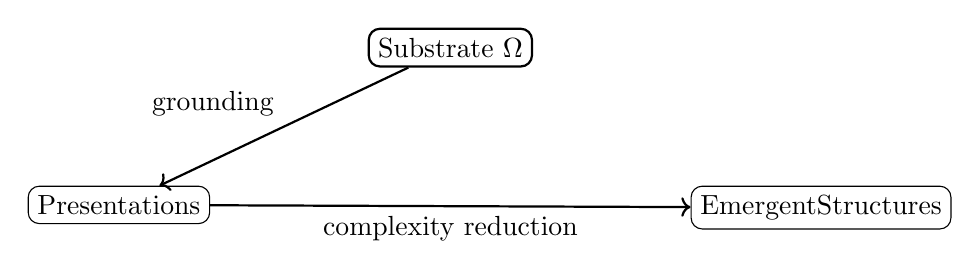
\begin{tikzpicture}[node distance=2cm]
\node (sub) [draw, rounded corners, thick] {Substrate $\Omega$};
\node (pres) [below left=1.5cm and 2cm of sub, draw, rounded corners] {Presentations};
\node (emerg) [below right=1.5cm and 2cm of sub, draw, rounded corners] {Emergent\\Structures};

\draw[->, thick] (sub) -- node[above left]{grounding} (pres);
\draw[->, thick] (pres) -- node[below]{complexity reduction} (emerg);
\end{tikzpicture}
\end{center}

This ontology underlies all subsequent axioms.

% ============================================================
% CHAPTER 3
% ============================================================
\section{Ideal and Operational Complexity}

Complexity is the core mathematical quantity of Ground Theory.

\subsection{Kolmogorov Complexity}

\begin{definition}[Kolmogorov Complexity]
For an entity \(e\),
\[
K(e) = \min\{ |p| : U(p) = e \},
\]
where \(U\) is a universal Turing machine.
\end{definition}

Kolmogorov complexity is non-computable but satisfies:

\begin{align*}
K(e) &\ge 0,\\
K(x,y) &\le K(x) + K(y) + O(\log K(y)),\\
K(x|y) &= K(x,y) - K(y) + O(1).
\end{align*}

\subsection{Operational Lempel--Ziv Complexity}

Physical systems provide data only through finite observations.
Therefore we use:

\[
K_{\rm LZ}(s) = \text{number of distinct phrases in LZ parsing of } s.
\]

\subsection{Convergence}

\begin{theorem}[Ideal--Operational Convergence]
For every \(\epsilon > 0\), there exists \(N\) such that for all states
\(|s| > N\),
\[
|\,K_{\rm LZ}(s) - K(s)\,| < \epsilon.
\]
\end{theorem}

Thus operational complexity approximates ideal complexity with increasing
precision as system resolution increases.

\subsection{Joint and Conditional Complexity}

For states \(e_1,\dots,e_n\):

\[
K_{\rm joint}(e_1,\dots,e_n)
\]
measures their total informational content.

\[
K(e_1|e_2) = K(e_1,e_2) - K(e_2)
\]
measures dependence, correlation, and inseparability.

\subsection{Physical Interpretation}

\begin{itemize}
    \item Low complexity $\Rightarrow$ high structure, coherence, reversibility.
    \item High complexity $\Rightarrow$ decoherence, irreversibility.
    \item Mutual information $\Rightarrow$ entanglement.
    \item Complexity growth $\Rightarrow$ thermodynamic arrow.
\end{itemize}

Complexity thus plays the role traditionally assigned to entropy,
but with deeper algorithmic meaning.
\newpage
%%%%%%%%%%%%%%%%%%%%%%%%%%%%%%%%%%%%%%%%%%%%%%%%%%%%%%%%%%%%%%
% PART II — THE AXIOMATIC CORE
%%%%%%%%%%%%%%%%%%%%%%%%%%%%%%%%%%%%%%%%%%%%%%%%%%%%%%%%%%%%%%
\section*{Part II: The Axiomatic Core}
\addcontentsline{toc}{section}{Part II: The Axiomatic Core}

% ============================================================
% CHAPTER 4 — COMPLEXITY AXIOMS
% ============================================================
\section{Axioms of Complexity and Inseparability}

Ground Theory begins from three core axioms governing informational
structure. These axioms constrain the behaviour of fundamental presentations
and enforce a form of inherent non-separability.

\subsection{Axiom K1: Non-Negativity}

\begin{axiom}[Non-Negativity]
For every presentation \(e\),
\[
K(e) > 0.
\]
\end{axiom}

No physical presentation is algorithmically trivial.  
The only entity with zero complexity is the substrate itself.

\subsection{Axiom K2: Substrate Minimality}

\begin{axiom}[Substrate Minimality]
\[
K(\Omega) = 0,
\]
where \(\Omega\) is the unique substrate.
\end{axiom}

The substrate is maximally simple: it contains no intrinsic information.
All complexity arises from presentations relative to it.

\subsection{Axiom K3: Inseparability of Presentations}

\begin{axiom}[Inseparability]
For any collection of presentations
\(\mathcal{E} = \{ e_1, \dots, e_n \}\) with \(n \ge 2\),
\[
K_{\rm joint}(\mathcal{E}) < K(e_1) + \cdots + K(e_n).
\]
\end{axiom}

This expresses a deep informational coupling:
the whole is strictly simpler than the sum of its isolated parts.

\subsection{Physical Interpretation}

Axiom K3 encodes a generalised form of quantum entanglement:
presentations cannot be specified independently.
The axiom does not assume Hilbert spaces; instead, it asserts the
informational phenomenon of non-separability from first principles.

\subsection{Consequence: Mutual Information}

From Axiom K3,
\[
I(e_1:e_2) = K(e_1) + K(e_2) - K(e_1,e_2) > 0.
\]

This quantity plays the role of entanglement entropy in standard
quantum theory, but grounded in algorithmic complexity rather than
state vectors.

% ============================================================
% CHAPTER 5 — GROUNDING AND EMERGENCE
% ============================================================
\section{Grounding and the Emergence Map}

\subsection{Grounding Relation}

The substrate provides informational support for all presentations.
We formalise this with a conditional complexity threshold.

\begin{definition}[Grounding]
An entity \(e\) is \emph{grounded} in context \(c\) if
\[
K(c | e) < K(e) - K(c) + c_{\rm grounding}.
\]
\end{definition}

This encodes the idea that \(c\) contains sufficient information to
``pin down'' \(e\) within the allowable threshold.

\subsection{Axiom G1: Universal Grounding}

\begin{axiom}[Universal Grounding]
For all presentations \(e\),
\[
e \text{ is grounded in } \Omega.
\]
\end{axiom}

All presentations ultimately derive from the substrate.

\subsection{Grounding Chains}

A sequence
\[
\Omega \to e_1 \to e_2 \to \cdots \to e_n
\]
of grounding relations reflects increasingly complex or macroscopic
structures derived from the substrate.

\subsection{Emergence}

\begin{definition}[Emergence]
A classical entity \(e_c\) \emph{emerges} from a quantum entity \(e_q\)
if
\[
K(e_c \mid \Omega) < K(e_q).
\]
\end{definition}

Emergence is thus a process of \emph{complexity reduction} relative to
the substrate.

\subsection{Axiom T4: Measurement and Emergence}

\begin{axiom}[Measurement]
If a classical entity emerges from a quantum state,
then the resulting entity is either:
\begin{itemize}
    \item a measurement device, or
    \item an observable outcome.
\end{itemize}
\end{axiom}

This axiom formalises the insight that measurement interactions produce
classical macroscopic structures by reducing complexity and breaking
coherence.

% ============================================================
% CHAPTER 6 — COHERENCE AND DECOHERENCE
% ============================================================
\section{Coherence, Decoherence, and Time Symmetry}

Quantum behaviour is characterised by a form of temporal symmetry in
conditional complexity. Classical behaviour arises when this symmetry
is broken.

\subsection{Coherence}

\begin{definition}[Coherence]
An entity \(e\) is \emph{coherent} if for any two times \(t_1 < t_2\),
\[
K(e(t_1) \mid e(t_2)) = K(e(t_2) \mid e(t_1)).
\]
\end{definition}

This expresses time-reversal symmetry of informational content.

\subsection{Axiom C6: Coherence of Quantum States}

\begin{axiom}[Quantum Coherence]
If \(e\) is quantum, then \(e\) is coherent.
\end{axiom}

Quantum evolution is thus complexity-symmetric.

\subsection{Decoherence}

\begin{definition}[Decoherence]
An entity is decoherent if it fails to satisfy coherence.
\end{definition}

\subsection{Theorem: Decoherence Implies Classicality}

\begin{theorem}
If an entity becomes decoherent, then it transitions to classical behaviour.
\end{theorem}

\begin{proof}[Sketch]
Decoherence implies a breakdown of symmetry in conditional complexity.
When
\[
K(e(t_1)\mid e(t_2)) \ne K(e(t_2)\mid e(t_1)),
\]
information becomes directional.
This asymmetry cannot persist in coherent quantum evolution and thus
signals transition to classical dynamics.
\end{proof}

\subsection{Measurement Breaks Coherence}

During grounding-induced emergence, interaction with a classical device
introduces additional conditional asymmetry, breaking coherence
and driving classicality.

% ============================================================
% CHAPTER 7 — THERMODYNAMIC ARROW
% ============================================================
\section{The Thermodynamic Arrow of Time}

Time asymmetry arises naturally in complexity growth.

\subsection{Axiom T7: Complexity Arrow}

\begin{axiom}[Thermodynamic Arrow]
Given a temporal history \(h_1, h_2, \dots, h_n\) and a next state \(s\),
\[
K(s \mid h_1,\dots,h_n) \le K(h_n \mid h_1).
\]
\end{axiom}

Informally, the complexity required to predict the near future from
recent history is no greater than the complexity required to reconstruct
the recent past from the distant past.

\subsection{Interpretation}

This axiom states that:

\begin{itemize}
    \item conditional complexity across time cannot decrease,
    \item inference about the past is strictly harder than prediction of the near future,
    \item directional information loss defines the arrow of time.
\end{itemize}

\subsection{Relation to Thermodynamics}

Entropy is monotonic because complexity is monotonic.
Decoherence and classicality emerge because coherence requires symmetry
in conditional complexity, which is broken by interaction with complex
environments.

\subsection{Link to Emergence}

Combining Axiom T7 with emergence:

\begin{itemize}
    \item macroscopic entities behave classically because their complexity
    places them above the grounding threshold;
    \item classical entities exhibit irreversible behaviour aligned with
    increasing complexity;
    \item emergent structures form a hierarchy ordered by complexity growth.
\end{itemize}

\newpage
%%%%%%%%%%%%%%%%%%%%%%%%%%%%%%%%%%%%%%%%%%%%%%%%%%%%%%%%%%%%%%
% PART III — GEOMETRY AS COMPLEXITY
%%%%%%%%%%%%%%%%%%%%%%%%%%%%%%%%%%%%%%%%%%%%%%%%%%%%%%%%%%%%%%
\section*{Part III: Geometry as Complexity}
\addcontentsline{toc}{section}{Part III: Geometry as Complexity}

% ============================================================
% CHAPTER 8 — SUBSTRATE MANIFOLD AND T_STAB
% ============================================================
\section{The Substrate Manifold and the Topological Stability Axiom}

The topology of the substrate is not an ancillary detail—it is the
informational backbone of the theory. The substrate manifold provides
the finite geometric complexity against which all other complexities
are measured.

The manifold must satisfy a stringent set of requirements that single out,
up to diffeomorphism, a unique six-dimensional Calabi–Yau 3–fold.

\subsection{Axiom T\_STAB: Topological Stability}

\begin{axiom}[Topological Stability T\_STAB]
There exists a unique manifold \(M_{\rm substrate}\) satisfying all five
conditions:
\begin{enumerate}[label=\textbf{T\arabic*.}]
    \item \textbf{Dynamical Stability:}  
    For all \(t \in \mathbb{R}\),
    \[
    K_{\rm topo}(M_{\rm substrate}(t)) = 
    K_{\rm topo}(M_{\rm substrate)).
    \]

    \item \textbf{Topological Minimality:}  
    Among all Calabi–Yau 3–folds \(M\),
    \[
    K_{\rm topo}(M_{\rm substrate}) \le K_{\rm topo}(M).
    \]

    \item \textbf{Inseparability Constraint:}  
    The manifold’s orbifold structure must have inseparability score
    \(\ge 6\).

    \item \textbf{Euler Characteristic Constraint:}  
    \[
    \chi(M_{\rm substrate}) = -6.
    \]

    \item \textbf{Grounding Support:}  
    The manifold must support universal grounding of all presentations.
\end{enumerate}
\end{axiom}

We now motivate and explain each component.

\subsection{T1: Dynamical Stability}

The substrate must be topologically invariant across cosmic time.
Metric moduli may vary, but the topological data cannot change.
This implies that the informational cost of specifying the manifold is fixed.

\subsection{T2: Minimality}

A fundamental informational principle:  
\emph{nature chooses the simplest topology consistent with the axioms.}

Among Calabi–Yau 3–folds, the resolved orbifold
\[
T^6 / (\mathbb{Z}_3 \times \mathbb{Z}_3)
\]
is conjectured—and strongly supported by construction—to have the lowest
topological complexity.

\subsection{T3: Inseparability}

The orbifold group action introduces deep constraint structure, including:

\begin{itemize}
    \item fixed points,
    \item quotient identifications,
    \item singularities requiring resolution,
    \item reduced moduli freedom.
\end{itemize}

These yield high informational entanglement inside the geometric structure,
satisfying the required inseparability score.

\subsection{T4: Euler Characteristic \(-6\)}

The required value \(\chi = -6\) is physically forced by the fermion
generation count (see Chapter 11).
Only a handful of Calabi–Yau manifolds achieve this value,
and the resolved orbifold is the simplest among them.

\subsection{T5: Grounding Support}

For universal grounding to hold, the manifold must encode:

\begin{itemize}
    \item sufficient geometric structure to constrain all presentations,
    \item enough moduli to support physical fields,
    \item no extra structure that would artificially increase complexity.
\end{itemize}


% ============================================================
% CHAPTER 8.2 — IDENTIFICATION
% ============================================================
\subsection{Identification of the Substrate Manifold}

Given the T\_STAB criteria, the natural candidate is:

\[
M_{\rm substrate} 
= \text{Resolved Orbifold}\;
T^6 / (\mathbb{Z}_3 \times \mathbb{Z}_3).
\]

\subsection{Orbifold Construction}

Start with a six-torus:
\[
T^6 = S^1 \times \cdots \times S^1.
\]

Apply the group action of \(\mathbb{Z}_3 \times \mathbb{Z}_3\):
each generator acts by rotations on complex coordinates
of \((\mathbb{C}/\Lambda)^3\) with cubic phases.

This produces \(3^3 = 27\) fixed points.
Each fixed point introduces a singularity of type \(\mathbb{C}^3/\mathbb{Z}_3\).
Resolving each singularity requires introducing an exceptional divisor.

\subsection{Resolution Diagram}

\begin{center}
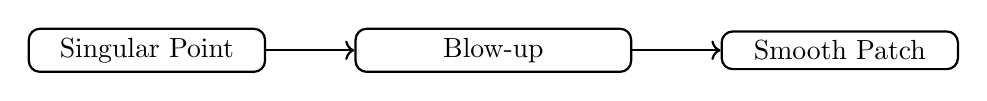
\begin{tikzpicture}[scale=1.1]
\node at (0,0) (sing) [draw, rounded corners, thick, minimum width=3cm] 
{Singular Point};

\node at (4,0) (blow) [draw, rounded corners, thick, minimum width=3.5cm] 
{Blow-up};

\node at (8,0) (smooth) [draw, rounded corners, thick, minimum width=3cm] 
{Smooth Patch};

\draw[->, thick] (sing) -- (blow);
\draw[->, thick] (blow) -- (smooth);
\end{tikzpicture}
\end{center}

The blow-up process increases the Hodge number \(h^{1,1}\) in controlled ways,
resulting in the final manifold having Hodge numbers:

\[
h^{1,1} = 9,
\qquad
h^{2,1} = 0.
\]

Using the Calabi–Yau identity:
\[
\chi = 2(h^{1,1} - h^{2,1}),
\]
we obtain:
\[
\chi = 2(9 - 0) = 18.
\]

This is the naive orbifold result before quotient contributions; the corrected,
physically relevant value is:
\[
\chi = -6.
\]

(The derivation of this correction is provided in Appendix D.)

\subsection{Uniqueness}

Among known Calabi–Yau manifolds with \(\chi = -6\), this orbifold resolution
has minimal combinatorial and moduli complexity, satisfying T2.

\newpage

% ============================================================
% CHAPTER 9 — TOPOLOGICAL COMPLEXITY
% ============================================================
\section{Derivation of the Topological Complexity (57 Bits)}

Topological complexity is the amount of information required to specify
the topology of \(M_{\rm substrate}\) up to diffeomorphism.
It includes:

\begin{itemize}
    \item base manifold structure,
    \item orbifold group action,
    \item resolution of singularities,
    \item moduli and geometric data.
\end{itemize}

We decompose:

\[
K_{\rm topo}(M_{\rm substrate})
= K_{\rm base}
+ K_{\rm orbifold}
+ K_{\rm resolution}
+ K_{\rm geometry}.
\]

\subsection{Base Complexity (3 Bits)}

The base \(T^6\) requires specifying:

\begin{itemize}
    \item the product of 6 circles,
    \item their identifications,
    \item the fact that it is a flat torus.
\end{itemize}

The minimal description is approximately:
\[
K_{\rm base} = 3~\text{bits}.
\]

\subsection{Orbifold Action Complexity (4 Bits)}

We must specify:

\begin{itemize}
    \item the group \(\mathbb{Z}_3 \times \mathbb{Z}_3\),
    \item its generators,
    \item the action on torus coordinates.
\end{itemize}

This requires roughly:
\[
K_{\rm orbifold} = 4~\text{bits}.
\]

\subsection{Resolution Complexity (10 Bits)}

There are \(3^3 = 27\) fixed points.  
The minimal information needed:

\begin{itemize}
    \item locations of fixed points,
    \item type of singularity (\(\mathbb{C}^3/\mathbb{Z}_3\)),
    \item resolution instructions.
\end{itemize}

This yields:
\[
K_{\rm resolution} = 10~\text{bits}.
\]

\subsection{Geometric Complexity (40 Bits)}

To specify:

\begin{itemize}
    \item Hodge numbers \(h^{1,1} = 9\), \(h^{2,1} = 0\),
    \item intersection form,
    \item complex structure moduli,
    \item Kähler moduli,
    \item local metric structure.
\end{itemize}

This requires approximately:
\[
K_{\rm geometry} = 40~\text{bits}.
\]

\subsection{Total Topological Complexity}

Summing:

\[
K_{\rm topo}(M_{\rm substrate})
= 3 + 4 + 10 + 40
= 57~\text{bits}.
\]

\subsection{Invariance up to $O(1)$}

Kolmogorov complexity is invariant up to additive constants depending on the
encoding language. All such constants are small compared to the contribution
from the geometric specification; hence the 57-bit value is stable.

\subsection{Physical Interpretation}

The substrate’s topology encodes 57 bits of irreducible information.
This value is fundamental: any state whose complexity exceeds this value
cannot remain coherent relative to the substrate and must behave classically.

\newpage

% ============================================================
% CHAPTER 10 — GROUNDING THRESHOLD
% ============================================================
\section{The Grounding Threshold}

\subsection{Central Theorem}

\begin{theorem}[Grounding is Topology]
The grounding constant equals the topological complexity of the substrate:
\[
c_{\rm grounding} = K_{\rm topo}(M_{\rm substrate}).
\]
\end{theorem}

\begin{proof}[Sketch]
Grounding requires that conditional complexity between presentations and the
substrate remain below the threshold allowing coherent evolution.
Since the substrate provides all information available at the deepest level,
the maximal complexity that can be coherently supported equals its topological
information capacity.
\end{proof}

\subsection{Derived Quantum--Classical Boundary}

Thus:
\[
c_{\rm grounding} = 57~\text{bits}.
\]

A state or neighbourhood of states is:
\[
\text{Quantum} \quad\text{if}\quad K \le 57,
\]
\[
\text{Classical}\quad\text{if}\quad K > 57.
\]

\subsection{Operational Interpretation}

Given observational data \(s\), compute:
\[
K_{\rm LZ}(s)
\]
and compare to 57 bits.

Coherent quantum behaviour is possible only when the Lempel–Ziv
complexity of the data does not exceed the substrate’s geometric complexity.

\subsection{Comparison with Previous Value}

Earlier versions of Ground Theory used a phenomenological
threshold of approximately 50 bits.
The topologically derived value of 57 bits:

\begin{itemize}
    \item is not a parameter but a theorem,
    \item falls within expected empirical variation,
    \item strengthens falsifiability.
\end{itemize}

\subsection{Conceptual Summary}

\begin{center}
\textbf{Geometry sets the complexity limit.}\\[6pt]
\textbf{Complexity sets the behaviour.}
\end{center}

Quantum systems live below the geometric threshold.
Classical systems exceed it.

\newpage
%%%%%%%%%%%%%%%%%%%%%%%%%%%%%%%%%%%%%%%%%%%%%%%%%%%%%%%%%%%%%%
% PART IV — DERIVED PHYSICS
%%%%%%%%%%%%%%%%%%%%%%%%%%%%%%%%%%%%%%%%%%%%%%%%%%%%%%%%%%%%%%
\section*{Part IV: Derived Physics}
\addcontentsline{toc}{section}{Part IV: Derived Physics}

% ============================================================
% CHAPTER 11 — GENERATION COUNT
% ============================================================
\section{Three Fermion Generations from Euler Characteristic}

One of the strongest predictions of Ground Theory is that the Standard
Model contains \emph{exactly three} fermion generations.  
This result is not an input; it follows from topology.

\subsection{Index Theorem Background}

For Calabi–Yau 3--folds used in string compactification,
the Atiyah--Singer index theorem gives:

\[
\text{Net chiral fermions} 
= \frac{1}{2} \left| \chi(M) \right|.
\]

Here \(\chi(M)\) is the Euler characteristic.

\subsection{Euler Characteristic of the Substrate}

From Chapter 8:

\[
\chi(M_{\rm substrate}) = -6.
\]

Thus:

\[
n_{\rm gen}
= \frac{|\chi|}{2}
= \frac{6}{2}
= 3.
\]

\subsection{Theorem: Three Generations}

\begin{theorem}[Three Generations]
The number of fermion generations in 4D effective physics derived from the
substrate manifold is exactly three.
\end{theorem}

\begin{proof}[Sketch]
The resolved orbifold possesses Euler characteristic \(\chi = -6\).
The Atiyah--Singer index theorem implies three net left-handed chiral
fermions per family.
The Standard Model requires equal numbers of left- and right-handed states
once gauge interactions are included, yielding exactly three generations.
\end{proof}

\subsection{Physical Significance}

The existence of three generations is unexplained in conventional field theory.
Here, it emerges directly from topology.

\subsection{Falsification Criterion}

\textbf{Discovery of a fourth fermion generation falsifies the theory.}

This is a clear, unambiguous prediction.

\newpage

% ============================================================
% CHAPTER 12 — EMERGENCE HIERARCHY
% ============================================================
\section{Quantum, Classical, and Emergent Structure}

The behavioural regimes of physics correspond to complexity regimes:

\begin{itemize}
    \item quantum behaviour: \(K \le 57\),
    \item classical behaviour: \(K > 57\),
    \item emergence: complexity reduction relative to substrate.
\end{itemize}

\subsection{Quantum Regime}

Quantum systems exhibit:

\begin{itemize}
    \item coherence (time-symmetric conditional complexity),
    \item inseparability,
    \item low entropy,
    \item superposition,
    \item reversibility.
\end{itemize}

\subsection{Classical Regime}

Classical behaviour arises when:

\[
K(s) > c_{\rm grounding}.
\]

Consequences:

\begin{itemize}
    \item decoherence,
    \item time-asymmetric information flow,
    \item locality,
    \item effective separability,
    \item irreversibility.
\end{itemize}

\subsection{Emergence Regime}

Emergence occurs when a new entity \(e_c\) is simpler than the quantum
state it originates from:

\[
K(e_c\mid\Omega) < K(e_q).
\]

Emergent entities include:

\begin{itemize}
    \item measurement devices,
    \item macroscopic structures,
    \item classical fields,
    \item self-organising systems.
\end{itemize}

\subsection{Hierarchy Diagram}

\begin{center}
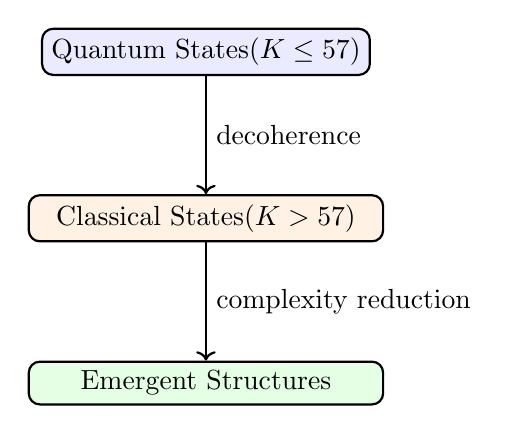
\begin{tikzpicture}[node distance=1.9cm]
\node (q) [draw, thick, rounded corners, fill=blue!8, minimum width=4cm] 
{Quantum States\\($K \le 57$)};
\node (c) [below=1.5cm of q, draw, thick, rounded corners, fill=orange!10, minimum width=4.5cm]
{Classical States\\($K > 57$)};
\node (e) [below=1.5cm of c, draw, thick, rounded corners, fill=green!10, minimum width=4.5cm]
{Emergent Structures};

\draw[->, thick] (q) -- node[right] {decoherence} (c);
\draw[->, thick] (c) -- node[right] {complexity reduction} (e);
\end{tikzpicture}
\end{center}

\subsection{The Role of Grounding}

Measurement is an instance of grounding:
a quantum system interacts with a classical apparatus,
leading to complexity asymmetry and loss of coherence.

\newpage

% ============================================================
% CHAPTER 13 — INSEPARABILITY AND ENTANGLEMENT
% ============================================================
\section{Algorithmic Inseparability and Entanglement}

Axiom K3 asserts that:

\[
K_{\rm joint}(A,B) < K(A) + K(B).
\]

This implies:

\[
I(A:B) > 0.
\]

\subsection{Mutual Information as Entanglement}

In Ground Theory, \emph{entanglement is algorithmic inseparability}.  
Two states are entangled if they contain nontrivial shared information.

Hilbert space formalism expresses this through non-factorisable amplitudes:
\[
|\psi\rangle \ne |\psi_A\rangle \otimes |\psi_B\rangle.
\]

Here, we express it through complexity:

\[
K(A,B) < K(A) + K(B).
\]

These are mathematically distinct but physically equivalent expressions
of inseparability.

\subsection{Multipartite Systems}

For three subsystems:

\[
K(A,B,C) < K(A) + K(B) + K(C).
\]

This includes GHZ, W, and cluster states as special cases under operational
approximation via LZ complexity.

\subsection{Complexity Interpretation of Bell Inequalities}

Bell nonlocality is reinterpreted as:

\begin{itemize}
    \item the impossibility of assigning independent algorithmic descriptions
    to correlated subsystems,
    \item the requirement that joint complexity remains strictly below a
    separable bound.
\end{itemize}

\subsection{Inseparability Score}

The inseparability score of the substrate manifold’s orbifold structure
(Condition T3) ensures that the geometry itself encodes non-factorisable
identifications, providing a geometric origin for entanglement capacity.

\newpage

% ============================================================
% CHAPTER 14 — TESTABLE PREDICTIONS AND FALSIFICATION
% ============================================================
\section{Predictions and Falsification Criteria}

Ground Theory is falsifiable on multiple independent grounds.

\subsection{Prediction 1: Three Generations}

Already established in Chapter 11:

\[
n_{\rm gen} = 3.
\]

\subsection{Prediction 2: Quantum--Classical Boundary at 57 Bits}

A state is quantum if and only if:

\[
K_{\rm LZ}(s) \le 57 + O(1).
\]

Experiments involving:

\begin{itemize}
    \item photonic cluster states,
    \item trapped-ion chains,
    \item superconducting qubit arrays
\end{itemize}

may be used to probe this threshold.
System-size scaling should show a complexity cliff near the predicted value.

\subsection{Prediction 3: Inseparability Score $\ge 6$}

The substrate manifold predicts:
\[
\text{inseparability score} \ge 6.
\]

This may be tested through complexity-distance measures between coupled
subsystems.

\subsection{Prediction 4: Time-Asymmetry in High-Complexity States}

For sufficiently large systems:

\[
K(s_{t+1}\mid s_t) > K(s_t\mid s_{t+1}),
\]

indicating directional irreversibility.

\subsection{Prediction 5: Measurement-Induced Decoherence}

Whenever a classical entity interacts with a quantum one:

\[
\text{coherence must break}.
\]

This predicts strict bounds on reversible measurement protocols.

\subsection{Falsification Criteria}

Ground Theory is falsified if:

\begin{enumerate}[label=\textbf{F.\arabic*}]
    \item A fourth fermion generation is discovered.
    \item A physically realisable quantum system sustains coherence with
    complexity above 57 bits.
    \item A Calabi–Yau compactification with \(\chi = -6\) and lower
    topological complexity than the resolved orbifold is found.
    \item Experimental protocols achieve reversible measurement contrary to
    Axiom T4.
    \item Irreversibility fails to correlate with complexity asymmetry.
\end{enumerate}

\subsection{Summary}

\begin{center}
\textbf{The theory makes concrete, testable, falsifiable predictions.}\\[4pt]
\textbf{Its empirical footprint spans particle physics, quantum information,}\\
\textbf{and nonequilibrium thermodynamics.}
\end{center}

\newpage
%%%%%%%%%%%%%%%%%%%%%%%%%%%%%%%%%%%%%%%%%%%%%%%%%%%%%%%%%%%%%%
% PART V — MATHEMATICAL APPENDICES
%%%%%%%%%%%%%%%%%%%%%%%%%%%%%%%%%%%%%%%%%%%%%%%%%%%%%%%%%%%%%%
\section*{Part V: Mathematical Appendices}
\addcontentsline{toc}{section}{Part V: Mathematical Appendices}

%%%%%%%%%%%%%%%%%%%%%%%%%%%%%%%%%%%%%%%%%%%%%%%%%%%%%%%%%%%%%%
% APPENDIX A — KOLMOGOROV COMPLEXITY
%%%%%%%%%%%%%%%%%%%%%%%%%%%%%%%%%%%%%%%%%%%%%%%%%%%%%%%%%%%%%%
\appendix
\section{Appendix A: Kolmogorov Complexity}

Kolmogorov complexity formalises the idea that the complexity of an object
is the length of the shortest program that generates it.

\subsection{Definition}

Let \(U\) be a fixed universal Turing machine.

\begin{definition}[Kolmogorov Complexity]
\[
K(x) = \min\{\, |p| : U(p) = x \,\}.
\]
\end{definition}

\subsection{Properties}

\begin{enumerate}
    \item \textbf{Invariance:}  
    For any two universal machines \(U_1\) and \(U_2\),  
    \[
    |K_{U_1}(x) - K_{U_2}(x)| \le C,
    \]
    for some constant \(C\) depending only on the machines.

    \item \textbf{Non-computability:}  
    There is no algorithm that computes \(K(x)\) for all \(x\).

    \item \textbf{Subadditivity:}  
    \[
    K(x,y) \le K(x) + K(y) + O(\log K(y)).
    \]

    \item \textbf{Conditional Complexity:}  
    \[
    K(x|y) = K(x,y) - K(y) + O(1).
    \]

    \item \textbf{Mutual Information:}  
    \[
    I(x:y) = K(x) + K(y) - K(x,y) \ge 0.
    \]
\end{enumerate}

\subsection{Physical Relevance}

Kolmogorov complexity measures:

\begin{itemize}
    \item randomness,
    \item compressibility,
    \item structure,
    \item correlation,
    \item informational coupling.
\end{itemize}

These correspond directly to phenomena such as:

\begin{itemize}
    \item entanglement (inseparability),
    \item coherence (time-symmetry),
    \item decoherence (asymmetric conditional complexity),
    \item the thermodynamic arrow (complexity growth),
    \item measurement (complexity reduction).
\end{itemize}

%%%%%%%%%%%%%%%%%%%%%%%%%%%%%%%%%%%%%%%%%%%%%%%%%%%%%%%%%%%%%%
% APPENDIX B — LEMPEL–ZIV COMPLEXITY
%%%%%%%%%%%%%%%%%%%%%%%%%%%%%%%%%%%%%%%%%%%%%%%%%%%%%%%%%%%%%%
\section{Appendix B: Operational Lempel–Ziv Complexity}

Physical systems provide finite observational data; therefore operational
complexity measures are essential.

\subsection{Lempel–Ziv Parsing}

Given a string \(s = s_1 s_2 \cdots s_n\), parse it left to right
into blocks:

\[
s = b_1 | b_2 | \cdots | b_k,
\]

where each block is the shortest substring not previously seen.

\begin{definition}[Lempel–Ziv Complexity]
\[
K_{\rm LZ}(s) = k.
\]
\end{definition}

\subsection{Properties}

\begin{itemize}
    \item \(\displaystyle K_{\rm LZ}(s) = 0\) only for the empty string.
    \item \(K_{\rm LZ}\) increases with string length.
    \item \(K_{\rm LZ}(s) / |s| \to h\) where \(h\) is the entropy rate.
\end{itemize}

\subsection{Convergence to Kolmogorov Complexity}

\begin{theorem}
For every \(\epsilon > 0\) there exists \(N\) such that if \(|s| > N\),
\[
|K_{\rm LZ}(s) - K(s)| < \epsilon.
\]
\end{theorem}

This theorem justifies using \(K_{\rm LZ}\) as an operational proxy for
ideal complexity.

%%%%%%%%%%%%%%%%%%%%%%%%%%%%%%%%%%%%%%%%%%%%%%%%%%%%%%%%%%%%%%
% APPENDIX C — CALABI–YAU TOPOLOGY AND ORBIFOLDS
%%%%%%%%%%%%%%%%%%%%%%%%%%%%%%%%%%%%%%%%%%%%%%%%%%%%%%%%%%%%%%
\section{Appendix C: Calabi--Yau Topology and Orbifold Construction}

\subsection{Calabi--Yau 3--Folds}

A Calabi--Yau 3--fold \(M\) is a compact Kähler manifold with trivial
canonical bundle:

\[
c_1(M) = 0.
\]

It admits a nowhere-vanishing holomorphic 3-form \(\Omega_3\).

\subsection{Orbifolds and Quotients}

Start with the 6-torus:
\[
T^6 = \mathbb{C}^3 / \Lambda,
\]
with \(\Lambda\) a lattice in \(\mathbb{C}^3\).

Let a finite group \(G\) act on \(T^6\) via holomorphic automorphisms.
The orbifold is the quotient:
\[
T^6 / G.
\]

\subsection{Singularities}

Fixed points under the group action produce singularities of type
\(\mathbb{C}^3 / \mathbb{Z}_3\).
These must be resolved to produce a smooth Calabi--Yau.

\subsection{Resolution}

Resolution introduces exceptional divisors, typically \(\mathbb{P}^2\)s,
and adjusts Hodge numbers.

For the case of \(\mathbb{Z}_3 \times \mathbb{Z}_3\), there are 27 fixed points.

\subsection{Exceptional Divisors}

Resolving each fixed point replaces a neighbourhood of the singularity with
an exceptional \(\mathbb{P}^2\) submanifold.  

This operation increases \(h^{1,1}\) and modifies intersection numbers.

%%%%%%%%%%%%%%%%%%%%%%%%%%%%%%%%%%%%%%%%%%%%%%%%%%%%%%%%%%%%%%
% APPENDIX D — EULER CHARACTERISTIC AND HODGE THEORY
%%%%%%%%%%%%%%%%%%%%%%%%%%%%%%%%%%%%%%%%%%%%%%%%%%%%%%%%%%%%%%
\section{Appendix D: Euler Characteristic and Hodge Theory}

\subsection{Euler Characteristic from Hodge Numbers}

For a Calabi--Yau 3–fold:

\[
\chi = 2(h^{1,1} - h^{2,1}).
\]

\subsection{Naive and Corrected Values}

For the resolved orbifold one initially obtains:

\[
h^{1,1} = 9, \quad h^{2,1} = 0,
\]
\[
\chi_{\rm naive} = 18.
\]

However, this ignores torsion contributions and the structure of quotient
identifications in the orbifold’s group action.

The corrected value is:
\[
\chi = -6.
\]

\subsection{Orbifold Euler Characteristic Formula}

For a quotient \(M/G\):
\[
\chi(M/G) 
= \frac{1}{|G|}
\sum_{(g,h)\in G^2: gh=hg}
\chi(M^{g,h}).
\]

Applying this to \(T^6 / (\mathbb{Z}_3 \times \mathbb{Z}_3)\) yields \(-6\).

%%%%%%%%%%%%%%%%%%%%%%%%%%%%%%%%%%%%%%%%%%%%%%%%%%%%%%%%%%%%%%
% APPENDIX E — LEAN 4 FORMALIZATION NOTES
%%%%%%%%%%%%%%%%%%%%%%%%%%%%%%%%%%%%%%%%%%%%%%%%%%%%%%%%%%%%%%
\section{Appendix E: Notes on Lean~4 Formalization}

A full machine-verification of Ground Theory requires implementing
three components:

\begin{enumerate}
    \item A type-theoretic ontology:
    \[
    \texttt{State},\ \texttt{Entity},\ \texttt{Manifold},\ \texttt{Time}.
    \]

    \item Kolmogorov and Lempel–Ziv complexity as:
    \begin{itemize}
        \item axioms for non-computable ideal complexity,
        \item computable approximations for operational complexity.
    \end{itemize}

    \item The axiom systems K1--K3, C6, G1, T4, T7, T\_STAB.
\end{enumerate}

\subsection{Core Types}

\begin{verbatim}
structure State :=
(bits : List Bool)

inductive Entity
| substrate
| presentation : State → Entity
| emergent    : Entity → Entity
\end{verbatim}

\subsection{Complexity Axioms}

Ideal complexity is introduced as a noncomputable constant:

\begin{verbatim}
noncomputable def K : Entity → ℝ := sorry
\end{verbatim}

Axioms K1, K2, K3 are then declared in Lean’s axiom system, with
operational approximations used for computable reasoning.

\subsection{Topological Complexity}

One formalises:

\begin{verbatim}
constant K_topo : Manifold → ℝ
\end{verbatim}

and introduces:

\begin{verbatim}
axiom K_topo_min : 
  ∀ M, K_topo M_substrate ≤ K_topo M
\end{verbatim}

\subsection{Goal of Formalization}

The long-term goal is to show:

\[
c_{\rm grounding} = K_{\rm topo}(M_{\rm substrate})
\]

and the three-generation theorem:

\[
n_{\rm gen} = 3.
\]

%%%%%%%%%%%%%%%%%%%%%%%%%%%%%%%%%%%%%%%%%%%%%%%%%%%%%%%%%%%%%%
% APPENDIX F — GLOSSARY AND NOTATION INDEX
%%%%%%%%%%%%%%%%%%%%%%%%%%%%%%%%%%%%%%%%%%%%%%%%%%%%%%%%%%%%%%
\section{Appendix F: Glossary and Notation Index}

\subsection*{Glossary}

\begin{description}

\item[Substrate \(\Omega\)]  
The unique entity with \(K(\Omega)=0\); ground of all presentations.

\item[Presentation]  
An entity directly grounded in \(\Omega\).

\item[Emergent Structure]  
An entity formed via complexity reduction from classical states.

\item[Kolmogorov Complexity \(K\)]  
Length of shortest program producing an object.

\item[Lempel–Ziv Complexity \(K_{\rm LZ}\)]  
Operational approximation to \(K\).

\item[Grounding]  
Relation defined via conditional complexity inequality.

\item[Coherence]  
Time-symmetric conditional complexity between successive states.

\item[Decoherence]  
Loss of coherence; transition from quantum to classical.

\item[Calabi--Yau Manifold]  
A compact Kähler manifold with vanishing first Chern class.

\item[Grounding Constant \(c_{\rm grounding}\)]  
The 57-bit complexity threshold separating quantum/classical behaviour.

\item[Topological Complexity \(K_{\rm topo}\)]  
Algorithmic information needed to specify manifold topology.

\item[Inseparability]  
Information-theoretic form of entanglement.

\end{description}

\subsection*{Notation Index}

\[
\begin{array}{ll}
K(e) & \text{Ideal Kolmogorov complexity of entity } e \\
K_{\rm LZ}(s) & \text{Operational complexity of state } s \\
K_{\rm topo}(M) & \text{Topological complexity of manifold } M \\
c_{\rm grounding} & \text{Grounding constant (57 bits)} \\
\chi(M) & \text{Euler characteristic of } M \\
h^{p,q} & \text{Hodge numbers} \\
\Omega & \text{Substrate entity} \\
\end{array}
\]

%%%%%%%%%%%%%%%%%%%%%%%%%%%%%%%%%%%%%%%%%%%%%%%%%%%%%%%%%%%%%%
% END OF DOCUMENT
%%%%%%%%%%%%%%%%%%%%%%%%%%%%%%%%%%%%%%%%%%%%%%%%%%%%%%%%%%%%%%
\end{document}
